\documentclass[twocolumn]{aastex61}

\newcommand{\vdag}{(v)^\dagger}
\newcommand\aastex{AAS\TeX}
\newcommand\latex{La\TeX}

\newcommand{\project}[1]{\textsl{#1}}
\newcommand{\JWST}{\project{JWST}}
\newcommand{\HST}{\project{HST}}
\newcommand{\Spitzer}{\project{Spitzer}}

%% Reintroduced the \received and \accepted commands from AASTeX v5.2
%\received{July 1, 2016}
%\revised{September 27, 2016}
%\accepted{\today}
\submitjournal{ApJ}

\shorttitle{Phase Curves of WASP-103b}
\shortauthors{Kreidberg et al.}

\begin{document}

\title{Phase Curves of WASP-103b}

\correspondingauthor{Laura Kreidberg}
\email{laura.kreidberg@cfa.harvard.edu}

\author{Laura Kreidberg}
\affiliation{Harvard Society of Fellows\
78 Mt. Auburn St.\\
Cambridge, MA 02138, USA}
\affiliation{Harvard-Smithsonian Center for Astrophysics\
60 Garden St.\\
Cambridge, MA 02138}
\nocollaboration

\author{Vivien Parmentier}
\affiliation{Department of Planetary Sciences and Lunar and Planetary Laboratory, The University of Arizona}
\nocollaboration

\author{Michael R. Line}
\affiliation{Arizona State University}
\nocollaboration

\author{Mick\"{a}el Bonnefoy}
\affiliation{Universit\'{e} Grenoble Alpes}
\nocollaboration

\author{Jacqueline K. Faherty}
\affiliation{American Museum of Natural History}
\nocollaboration

\author{Kevin B. Stevenson}
\affiliation{Space Telescope Science Institute}
\nocollaboration

\author{Gregory L. Henry}
\affiliation{Center of Excellence in Information Systems, Tennessee State University}
\nocollaboration

\author{Keivan Stassun}
\affiliation{Vanderbilt University}
\nocollaboration

\author{Jacob L. Bean}
\affiliation{University of Chicago}
\nocollaboration

\author{Jonathan Fortney}
\affiliation{University of California Santa Cruz}
\nocollaboration

\author{Adam Showman}
\affiliation{Department of Planetary Sciences and Lunar and Planetary Laboratory, The University of Arizona}
\nocollaboration

\author{Jean-Michel D\'{e}sert}
\affiliation{University of Amsterdam}

\begin{abstract}
WASP-103b is a short-period hot Jupiter.
\end{abstract}

\keywords{planets and satellites: individual (WASP-107b), planets and satellites: atmospheres}


\section{Introduction} \label{sec:intro}
It is a truism to say that planets are round.  The. And yet planets' roundness gives rise to a host of complications:  atmospheric circulation, variable , gradients in chemistry, cloud formation and evaporation, and time-dependent phenomena (weather).

It is a challenge is to reveal this structure at great distances, when we cannot spatially resolve the photosphere of the planet.  Most observations of exoplanet atmospheres are sensitive to a single isolated region  -- either the terminator, for transmission spectroscopy, or the disk-integrated dayside, for emission spectroscopy.  The solution to this problem is to observe phase curves of tidally-locked planets, which monitor the brightness of the planet over its entire orbit. As the orbital phase changes, the observer 

The first phase curve was observed with \Spitzer\ for the hot Jupiter HD 189733b by \citep{knutson??}, and was followed by FIXME more (with IRAC). Several trends emerged from these measurements, including eastward shifted hotspots (which suggest super-rotating equatorial jets), larger day-night temperature contrast for shorter period planets (ref), . The first spectroscopic phase curve was measured with Hubble's Wide Field Camera 3 (WFC3) by \citep{stevenson???} for the hot Jupiter WASP-43b. Found low albedo, offset hotspot, water visible at other phases, 

In parallel with these observations, there have been major advances in the theory of exoplanet atmospheres in three-dimensions. Global circulation models (GCMs) are now capable of self-consistent radiative transfer and atmospheric dynamics (refs) and are beginning to include clouds (refs?). 

In addition to GCMs, work on the inverse problem Cowan - how to get maps, . SPIDERMAN, an open-source Python package designed to take any temperature or brightness map of a planet and output the corresponding phase curve, so that we can readily connect GCMs to phase curve observations.  


In this paper we present \HST\ and \Spitzer\ phase curve observations of WASP-103b, a hot Jupiter with a mass of X, radius of Y, period of Z (cite discovery paper). These properties are similar to WASP-43b, except that WASP-103b has a much (FIXME vs FIXME K) thanks to its hot F?? star host. By comparing the phase curves of these two planets, we can test the effect of irradiation on the climate of the planet.

The structure of the paper is as follows:

\section{Observations and Data Reduction}
We observed two full-orbit phase curves of WASP-103b with \HST/WFC3 and one each with \Spitzer/IRAC at 3.6 and 4.5 $\mu$m (from HST Program 14050 and Spitzer Program 11099). We also reduced two \HST/WFC3 secondary eclipse observations of WASP-103b from \HST\ Program 13660 (PI: M. Zhao).

\subsection{\HST/WFC3}
The \HST\ phase curve observations consisted of two visits on 26-27 February and 2-3 August 2015. Each visit was 15 orbits in duration and spanned 23 hours. We took a direct image of the star with the F126N filter at the beginning of each orbit to determine the wavelength solution zero-point. The remainder of the orbit consisted of time-series spectroscopy with the G141 grism ($1.1 - 1.7$ $\mu$m) and the 256 x 256 pixel subarray. We used the SPARS10/NSAMP = 15 read-out mode, which has an exposure time of 103 seconds. To optimize the duty cycle of the observations, we used the spatial scan observing mode with a scan rate of 0.03"/s, alternating between forward and backward scanning on the detector. The scan height was 25 pixels and the peak counts were 35k photoelectrons per pixel. We collected a total of 18 spatial scan exposures per orbit.  The two eclipse observations from Program 13660 had a similar observing setup.  

We reduced the data from both programs using a custom pipeline developed for past analyses of WFC3 data \citep[for details see][]{kreidberg14a, kreidberg14b, kreidberg15a}. Briefly, we use the optimal extraction algorithm of \cite{horne86} to extract each up-the-ramp sample (or ``stripe") separately. The stripes are then summed to create the final spectrum. For each stripe, the extraction window is 24 pixels high and centered on the stripe midpoint. We estimate the background from the median of a region of the detector that is uncontaminated by the target spectrum (rows 5-50). The typical background counts are low (10-15 photoelectrons per pixel, roughly 0.03\% of the peak counts from the target star). We note that the extracted spectrum includes flux from a nearby star, which is separated from WASP-103 by less than two pixels \citep[0.2";][]{wollert15}. Our extracted spectrum includes flux from this star, which we account for later in the analysis. 

\subsection{\Spitzer}
The \Spitzer\ observations had the following setup. Each phase curve observation consisted of 30 hours of time series photometry, beginning three hours prior to one secondary eclipse and ending three hours after a second eclipse.  We used 12 s exposures to maximize the duty cycle without saturating the detector. The data volume is relatively low for this exposure time, so we read out the full array. To minimize the intrapixel effect (variations in flux caused by imprecise pointing), we did not dither and also used PCRS peak-up to improve the pointing accuracy. We began each observations with a 30-minute position settling period, followed by three Astronomical Observation Requests (AORs) of equal duration. At the beginning of each AOR, the telescope was repointed to position the target in the ``sweet spot" of the detector.

The data were reduced with the POET pipeline \citep{stevenson12}. We performed aperture photometry with an aperture size of 2.75 pixels (chosen from a grid of apertures between 2 and 4 pixels to minimize the residual noise in the light curve fits). We masked pixels that were flagged in the bad pixel mask provided in the ancillary data for the observations. The target centroid was determined with a two-dimensional Gaussian fit.  We estimated and subtracted the background from an annulus with a radius of 7 to 15 pixels from the centroid. As for the \HST\ observations, the contaminating flux from the nearby star is included in the final photometry and corrected later in the light curve fits.


\subsection{Photometric Monitoring}
We monitored WASP-103's photometric variability over 158 nights during 2014 - 2016 with the Tennessee State University Celestron 14-inch (C14) automated imaging telescope (AIT), located at Fairborn Observatory in southern Arizona \citep[see, e.g.,][]{h1999, ehf2003}.  The observations of WASP-103 were made in the Cousins R passband with an SBIG STL-1001E CCD camera.  Each observation consisted of 4--10 consecutive exposures on WASP-103 along with several dozen comparison stars in the same field. The individual consecutive frames were co-added and reduced to differential magnitudes (i.e., WASP-103 minus the mean brightness of the six best comparison stars). The nightly observations were corrected for bias, flat-fielding, pier-side offset, and differential atmospheric extinction.  

The photometric analyses are summarized for each observing season in Table\,\ref{tab:photometry}.  The standard deviation of WASP-103's brightness in each season is given in column~4.  The mean of the three standard deviations is 0.0058~mag, which is very comparable to the mean standard deviation of the six comparison stars (0.0055~mag).  To maximize the possibility of detection WASP-103's rotation, we normalized the photometry such that each observing season has the same mean, thereby removing long-term variability in WASP-103 and/or the comparison stars. We performed a periodogram analysis of the normalized dataset. Figure\,\ref{fig:photometry} shows the frequency spectrum and the phase curve computed with the best frequency, respectively.  We also performed a least-squares fit to the data to determine the best fit sine curve. The best fit period is 6.814 days, which agrees closely with the estimated stellar rotation period of 6.855 days \citep{getal2014}.  The variability amplitude is 0.005~mag, which has FIXME impact on our analysis here.

%The apparent low amplitude variability is likely due to rotational modulation in the visibility of weak, magnetic surface features \citep[see, e.g.,][]{hfh1995}.

%This implies there can be very little night-to-night variability in WASP-103. The three seasonal mean brightness values given in column 5 scatter about their grand mean with a standard deviation of 0.0036 mag, but we note that the most discrepant mean is from the third season, for which we have only partial coverage. Therefore, our results do not completely rule out low-level, year-to-year variability of 0.001~mag or so.

%We performed periodogram analyses of the individual observing seasons and the complete dataset and found no significant periodicity.  To maximize the possibility of detecting a rotation signal in WASP-103, we normalized the dataset by adding a constant offset to the second and third observing seasons to have the same mean as the first. 
%To first order, this removes possible long-term variability in WASP-103 and/or the comparison stars as well as any uncorrected, long-term systemmatic effects.  It is the normalized data that are plotted in the top panel of Fig.~1.


%We performed a least-squares fit to the data with a sine curve with trial frequencies between 0.005 and 0.95 c/d, corresponding to periods between one and 200 days. The goodness of fit at each frequency is measured as the reduction factor in the variance of the original data.  The result suggests low-amplitude brightness variability in WASP-103 with a period near 6.814 days. 


\begin{figure}
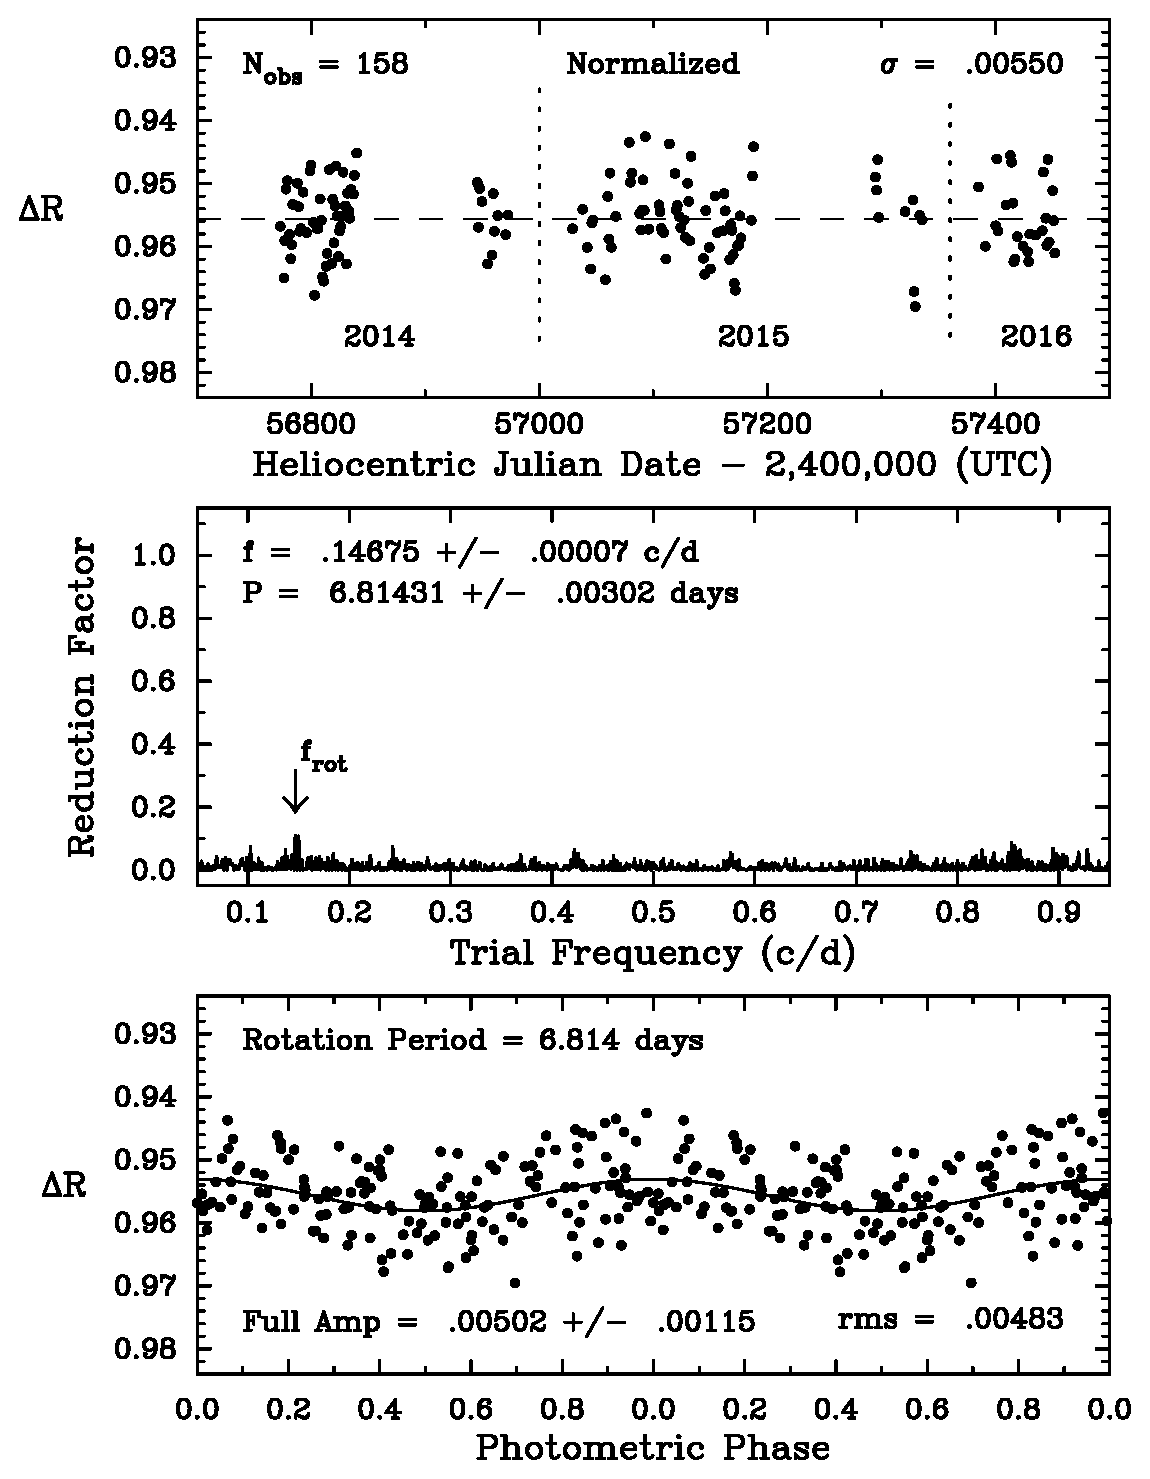
\includegraphics[width = 0.5\textwidth]{Figures/photometry.eps}
\caption{$Top$: The normalized nightly Cousins $R$ band photometric dataset for WASP-103, acquired with the C14 automated imaging telescope at Fairborn Observatory. Vertical dashed lines denote separate observing seasons. Gaps are due to target visibility and the Arizona monsoon season (July - September). $Middle$: The frequency spectrum of the normalized dataset suggests low-amplitude variability with a period of 6.814~days. $Bottom$: The normalized dataset phased to the 6.814-day period, which we interpret as the stellar rotation period. A least-squares sine fit to the 6.814-day rotation period gives a peak-to-peak amplitude of just 0.005~mag.}
\label{fig:photometry}
\end{figure}

\begin{deluxetable}{ccccc}
	%\tabletypesize{\small}
	\tablenum{1}
	\tablewidth{0pt}
	\tablecaption{Summary of Photometric Observations of WASP-103}
	\tablehead{
		\colhead{Observing} & \colhead{} & \colhead{Date Range} &
		\colhead{Sigma} & \colhead{Seasonal Mean}  \\

		\colhead{Season} & \colhead{$N_{obs}$} & \colhead{(HJD $-$ 2,400,000)} &
		\colhead{(mag)} & \colhead{(mag)}}%   \\

	%	\colhead{(1)} & \colhead{(2)} & \colhead{(3)} &
	%	\colhead{(4)} & \colhead{(5)}  
	\startdata
	   2014   &  59 & 56722--56972 & 0.0057 & $0.9546\pm0.0007$  \\
	   2015   &  73 & 57028--57335 & 0.0062 & $0.9549\pm0.0007$  \\
	   2016   &  26 & 57385--57451 & 0.0055 & $0.9485\pm0.0011$  \\
	\enddata
	\label{tab:photometry}
\end{deluxetable}


\subsection{Retrieval}


\section{Light Curve Fits}
which orbits/data
ellipsoidal variations/doppler beaming

\subsection{Phase-Resolved Spectra}

\subsection{Comparison of Thermal Phase Variation Models}

The raw data exhibit time-dependent systematic trends typically seen in WFC3 light curves, which we correct using a systematics model of the form:

\begin{equation}
 F_\mathrm{sys}(t) = (c\,S(t) + v_1\,t_\mathrm{v} + v_2\,t_\mathrm{v})(1 - \exp(-a\,t_\mathrm{orb} - b))
\end{equation}

\noindent where $t_\mathrm{v}$ is time elapsed since the first exposure in a visit and $t_\mathrm{orb}$ is time since the first exposure in an orbit. $S(t)$ is a scale factor equal to 1 for exposures with spatial scanning in the forward direction and $s$ for reverse scans. In the fit, $c$, $v_1$, $v_2$, $a$, $b$, and $s$ are free parameters. The first orbit in each visit shows larger systematic trends than subsequent orbits, so we exclude these data in our final analysis \citep[a common practice; see e.g.][]{kreidberg14a}.

We fit the systematics model simultaneously with the physical parameters for the system. The complete model is

\begin{equation}
F(t) = F_\mathrm{sys}(t)\left[T(t) + (E(t) - 1)(1 + A\cos(2\pi(t - \theta)/P))\right]
\label{eq:model}
\end{equation}

\noindent where $T(t)$ is a transit model, $E(t)$ is an eclipse model, $P$ is the planet orbital period, and $A$ and $\theta$ are free parameters to fit the amplitude and offset for the thermal phase variation. The free parameters for the transit and eclipse model are the planet-to-star radius ratio $r_p/r_s$, the planet-to-star flux ratio $f_p/f_s$, and a linear limb darkening parameter. The eclipse model is normalized such that the flux during eclipse is 1 and out of eclipse is $f_p/f_s$, and the transit model is normalized to unity out of transit. The planet's orbital parameters are poorly constrained by the WFC3 light curve due to incomplete phase coverage, so we fix the inclination to $i = 84.54^\circ$, the semi-major axis to stellar radius $a/R_s  = 2.925$, based on the best fit to the \emph{Spitzer} Channel 2 light curve (described below).  We use the orbital period $P = 0.925545613$ day, and time of inferior conjunction $t_0 = 2456836.2964455$ from \cite{southworth15}.  All free parameters were assumed to have a common value for both \emph{HST} visits, with the exception of $c$, $v_1$ and $v_2$, which were allowed to vary between visits. We explored adding an additional cosine term to model the thermal phase variation, but the additional degrees of freedom are not justified according to the Bayesian Information Criterion (BIC). The transit and eclipse models were calculated with the \texttt{batman} package \citep{kreidberg15a}. %Figure\;\ref{fig:w103_hst} shows the fitted broadband phase curve.

and fit the systematics with the BLISS mapping technique \citep{stevenson12}. This technique creates a map of the intrapixel sensitivity while simultaneously fitting for other systematics and the physical parameters of the system. In addition to the intrapixel sensitivity map, we fit the data for a linear trend in time and used the same transit, eclipse, and phase variation model as in Equation%\;\ref{eq:model}.


\section{Composition of the Atmosphere}

\subsection{Retrieval}

\section{Comparison with GCMs}

\section{Comparison with Brown Dwarfs and Directly Imaged Planets}


\acknowledgments
We thank a lot of people. Caroline Morley, Thomas Beatty, Ming Zhao, Kim Star Cartier, Hannah Diamond-Lowe, Nick Cowan (make him a coauthor?)

\bibliographystyle{aasjournal}
\bibliography{ms.bib}

\end{document}

